% -*- coding: UTF-8 -*-
% vim: autoindent expandtab tabstop=4 sw=4 sts=4 filetype=tex
% vim: spelllang=de spell
% chktex-file 27 - disable warning about missing include files

\chapter{Software-Architektur}
\label{chap:software-architecture}

\todo[inline]{Describe software architecture.}

Als Grundlage zur Entwicklung der Software-Architektur
dient~\citetitle{larman_applying_2004} von~\citeauthor{larman_applying_2004}.

Da~\cite{larman_applying_2004} auf dem Unified Process
(UP)~\cite{jacobson_unified_1999} basiert, wird vor allem dieser angewendet.
Dies hat ein iteratives Arbeiten zur Folge, da sich der UP auf agile Ansätze
wie Extreme Programming (XP) und Scrum fokussiert.

\todo[inline]{Describe general process}.
Process overview:
\begin{itemize}
    \item{Requirements}
    \item{Use cases}
    \item{Domain Models}
    \item{System Sequence Diagrams}
    \item{Packages}
    \item{Sequence Diagrams}
    \item{Class Diagrams}
    \item{Activity Diagrams}



% Sofern im Text nicht anders vermerkt, basiert das folgende Kapitel
% auf~\cite[S. 721ff]{foley_computer_1996}.
% 
% Für die Erzeugung und Darstellung von Bildern werden zwei Angaben
% benötigt: Was dargestellt werden soll und wie dieses dargestellt werden
% soll.
% Prinzipiell geht es darum zu bestimmen, welche Farbe eine Oberfläche an
% einem bestimmten Punkt hat. Dabei haben sich die Begriffe des
% \textit{Beleuchtungsmodelles (illumination model)} und des
% \textit{Modelles zur Schattierung (shading model)} etabliert.
% 
% \citeauthor{foley_computer_1996} nutzt den Begriff \textit{shading
% model} als Überbegriff~\parencite[S. 721]{foley_computer_1996}. Dieser
% schliesst auch Beleuchtungsmodelle ein.  Ein \textit{shading model}
% definiert, wann und mit welchen Parametern ein Beleuchtungsmodell
% angewendet wird. So nutzen manche \textit{shading models} ein
% Beleuchtungsmodell für jeden Pixel, andere wiederum nur für einzelne
% Pixel und interpolieren dabei die Werte der anderen Pixel.

% \input{inc/50/51_illumination_models}
% \input{inc/50/52_shading}

% -*- coding: UTF-8 -*-
% vim: autoindent expandtab tabstop=4 sw=4 sts=4 filetype=tex
% vim: spelllang=de spell
% chktex-file 27 - disable warning about missing include files

\section{Anforderungen}
\label{sec:requirements}

\subsection{Vision}
\label{subsec::requirements:vision}

Der Autor dieser Projektarbeit stellt sich eine Software zur Verwaltung und
Darstellung von Echtzeit-Animationen vor. Die Software soll es Anwendern erlauben
Echtzeit-Animationen in intuitiver Weise zu erstellen. Sie soll zudem modular
gehalten sein, so dass spätere Änderungen, wie z.B.\ zusätzliche Arten von
Rendering, ohne Weiteres adaptierbar sind.

\todo[inline]{Insert GUI mock-up here}

\subsection{Hauptkomponenten}
\label{subsec::requirements:main-components}

Die Applikation besteht aus zwei Applikationen: Einem \textit{Player},
welcher dem Abspielen von Echtzeit-Animationen dient, sowie einem \textit{Editor},
welcher der Erstellung und Verwaltung von Echtzeit-Animationen dient.

Der \textit{Editor} erlaubt den Export von erstellten Animationen inklusive den
dazugehörigen Dateien, wie zum Beispiel Bitmaps oder Modellen. Der
\textit{Player} kann die exportierten Animationen dann lesen und wiedergeben.

\subsection{Akteure (actors)}
\label{subsec::requirements:actors}

\textit{Primäre Akteure}
\begin{itemize}
    \item{%
            \textbf{Anwender}\\
            Ein \textit{Anwender} erstellt Echtzeit-Animationen mit der
            Software. Er hat also eine aktive Rolle.
        }
    \item{%
            \textbf{Betrachter}\\
            Ein \textit{Betrachter} nutzt die Software um eine durch den
            \textit{Anwender} erstellte Echtzeit-Animation anzusehen. Er nimmt
            also eine passive Rolle ein.
        }
\end{itemize}
\textit{Sekundäre Akteure}
\begin{itemize}
    \item{%
            \textbf{Entwickler}\\
            Ein \textit{Entwickler} erweitert die Software um neue Elemente
            (wie z.B.\ neue Shader).
        }
\end{itemize}

% -*- coding: UTF-8 -*-
% vim: autoindent expandtab tabstop=4 sw=4 sts=4 filetype=tex
% vim: spelllang=de spell
% chktex-file 27 - disable warning about missing include files

\subsection{Use Cases}
\label{subsec:requirements:use-cases}

Bei Use Cases handelt es sich um Anforderungen, genauer gesagt um funktionelle
bzw. Anforderungen an das Verhalten eines Systems~\cite[S. 61 bis 63]{larman_applying_2004}.
Sie sagen also aus, was ein System tut beziehungsweise tun soll. Die nachfolgenden Use
Cases sind keinesfalls vollständig --- dann wäre der Sinn des UP bzw.\ eines
iterativen Vorgehens verfehlt. Sie entwickeln sich viel mehr über die Zeit mit
dem Fortschreiten der Umsetzung (welche vor allem in der darauffolgenden
Projektarbeit statt findet).

Die Use Cases 1 bis und mit 5 sind bewusst sehr grob gehalten. Sie
veranschaulichen den Gesamtprozess. Use Cases 6 bis 10 zeigen den Prozess zur
Erstellung einer neuen Szene sowie einer Animation mehr im Detail.

\begin{longtabu}{p{0.2\textwidth}p{0.8\textwidth}}
    \centering\\
    \caption{Übersicht der Use Cases.}\label{table:uc-explanation}\\
    \toprule
        \textbf{Use Case 1} &
        Zeigt, wie ein Betrachter mittels Player eine Echtzeit-Animation
        betrachtet.\\
    \cmidrule(r){1-1}\cmidrule(lr){2-2}
        \textbf{Use Case 2} &
        Zeigt, wie ein Anwender mittels Editor eine Echtzeit-Animation
        erstellt.\\
    \cmidrule(r){1-1}\cmidrule(lr){2-2}
        \textbf{Use Case 3} &
        Zeigt, wie ein Anwender mittels Editor eine bestehende Echtzeit-Animation
        bearbeitet.\\
    \cmidrule(r){1-1}\cmidrule(lr){2-2}
        \textbf{Use Case 4} &
        Zeigt, wie ein Anwender mittels Editor eine Echtzeit-Animation
        für die Verwendung im Player exportiert.\\
    \cmidrule(r){1-1}\cmidrule(lr){2-2}
        \textbf{Use Case 5} &
        Zeigt, wie ein Entwickler neue Elemente, wie zum Beispiel Objekte oder
        Operationen, für den Editor bereitstellen kann.\\
    \cmidrule(r){1-1}\cmidrule(lr){2-2}
        \textbf{Use Case 6} &
        Zeigt im Detail, wie ein Anwender mittels Editor eine neue Szene
        erstellt.\\
    \cmidrule(r){1-1}\cmidrule(lr){2-2}
        \textbf{Use Case 7} &
        Zeigt im Detail, wie ein Anwender mittels Editor einen neuen Knoten zu
        einer bestehenden Szene hinzufügt.\\
    \cmidrule(r){1-1}\cmidrule(lr){2-2}
        \textbf{Use Case 8} &
        Zeigt im Detail, wie ein Anwender Knoten einer Szene mittels Graphen
        des Editors verbindet.\\
    \cmidrule(r){1-1}\cmidrule(lr){2-2}
        \textbf{Use Case 9} &
        Zeigt im Detail, wie ein Anwender ein Schlüsselbild für einen Parameter
        eines Knotens einer Szene des Editors erstellt.\\
    \cmidrule(r){1-1}\cmidrule(lr){2-2}
        \textbf{Use Case 10} &
        Zeigt im Detail, wie die Auswertung und Darstellung eines Knotens,
        sowohl im Editor als auch im Player, geschieht.\\
    \bottomrule
\end{longtabu}

Einleitend folgt eine Tabelle zur Erklärung der einzelnen Begriffe in den
nachfolgenden Use Cases.

% -*- coding: UTF-8 -*-
% vim: autoindent expandtab tabstop=4 sw=4 sts=4 filetype=tex
% vim: spelllang=de spell
% chktex-file 27 - disable warning about missing include files

\begin{longtabu}{p{0.3\textwidth}p{0.7\textwidth}}
    \centering\\
    \caption{Erklärung der Begrifflichkeiten der Use
        Cases, angelehnt an~\cite[S.
        67]{larman_applying_2004}.}\label{table:uc-explanation}\\
    \toprule
        \textbf{Bereich} &
        Der Bereich des Use Cases. Dies ist entweder der Editor oder aber der
        Player (siehe hierzu auch~\autoref{subsec:requirements:vision}).\\
    \cmidrule(r){1-1}\cmidrule(lr){2-2}
        \textbf{Stufe (level)} &
        ``Ziel des Benutzers'' oder ``Unterfunktion''.\\
    \cmidrule(r){1-1}\cmidrule(lr){2-2}
        \textbf{Primärer Aktor} &
        Primärer Aktor des Use Cases: Anwender, Betrachter oder Entwickler.
        Siehe auch~\autoref{subsec:requirements:actors}. \\
    \cmidrule(r){1-1}\cmidrule(lr){2-2}
        \textbf{Stakeholder und Interessen} &
        Interessenten des Use Cases und deren Ziele.\\
    \cmidrule(r){1-1}\cmidrule(lr){2-2}
        \textbf{Erfolgsszenario} &
        Typisches, gewünschtes Szenario des Uses Cases, bei welchem keinerlei
        Fehler oder Nebenwirkungen auftreten.\\
    \cmidrule(r){1-1}\cmidrule(lr){2-2}
        \textbf{Fehlerfall} &
        Zusätzliche, fehlerhafte Szenarien.\\
    \cmidrule(r){1-1}\cmidrule(lr){2-2}
        \textbf{Erweiterungen} &
        Zusätzliche Szenarien.\\
    \cmidrule(r){1-1}\cmidrule(lr){2-2}
        \textbf{Zusätzliche Anforderungen} &
        Non-funktionelle Anforderungen, welche in Relation zu dem Use Case
        stehen.\\
    \bottomrule
\end{longtabu}

% -*- coding: UTF-8 -*-
% vim: autoindent expandtab tabstop=4 sw=4 sts=4 filetype=tex
% vim: spelllang=de spell
% chktex-file 27 - disable warning about missing include files

\begin{table}[H]
    \centering
    \caption{Use Case UC1: Betrachten einer Echtzeit-Animation.}\label{table:uc1-watch-demo}
    \begin{tabular}{p{0.5\textwidth}p{0.5\textwidth}}
        \toprule
            \textbf{Bereich} &
            Player\\
        \cmidrule(r){1-1}\cmidrule(lr){2-2}
            \textbf{Level} &
            Ziel des Benutzers \\
        \cmidrule(r){1-1}\cmidrule(lr){2-2}
            \textbf{Primärer Aktor} &
            Betrachter \\
        \cmidrule(r){1-1}\cmidrule(lr){2-2}
            \textbf{Stakeholder und Interessen} &
            Betrachter: Möchte eine zuvor erstellte Echtzeit-Animation ansehen.  \newline
            Anwender: Testen einer erstellen Echtzeit-Animation. \newline
            Entwickler: Testen einer erstellen Echtzeit-Animation. \\
        \cmidrule(r){1-1}\cmidrule(lr){2-2}
            \textbf{Erfolgsszenario} &
            \begin{enumerate}
                \item{Der Betrachter startet die Player-Applikation und wählt
                        die gewünschten Optionen, wie Auflösung und Bit-Tiefe.}
                \item{Der Betrachter startet die Animation.}
                \item{Der Player spielt die Animation bis zum Ende.}
                \item{Der Player wird automatisch geschlossen.}
            \end{enumerate} \\
        \cmidrule(r){1-1}\cmidrule(lr){2-2}
            \textbf{Erweiterungen} &
            \begin{enumerate}[label= (\alph*)]
                \item{Vorzeitiger Abbruch durch den Betrachter
                    \begin{enumerate}[label= (\roman*)]
                            \item{Der Betrachter bricht eine laufende Animation
                                    ab.}
                            \item{Der Player wird sofort geschlossen.}
                    \end{enumerate}
                }
                \item{Absturz/Ausfall des Systems
                    \begin{enumerate}[label= (\roman*)]
                            \item{Das System stürzt an einem beliebigen Punkt
                                    ab.}
                            \item{Neustart des Players.}
                            \item{Der Player beginnt die Animation von vorne.}
                    \end{enumerate}
                }
            \end{enumerate}
            \\
        \cmidrule(r){1-1}\cmidrule(lr){2-2}
            \textbf{Zusätzliche Anforderungen} &
            \todo[inline]{Add add. requirements} \\
        \bottomrule
    \end{tabular}
\end{table}


% -*- coding: UTF-8 -*-
% vim: autoindent expandtab tabstop=4 sw=4 sts=4 filetype=tex
% vim: spelllang=de spell
% chktex-file 27 - disable warning about missing include files

\subsubsection{Use Case UC2: Erstellen einer Echtzeit-Animation}
\label{ssubsec:requirements:use-cases:uc2}

\begin{longtabu}{p{0.5\textwidth}p{0.5\textwidth}}
    \centering\\
    \caption{Use Case UC2: Erstellen einer
        Echtzeit-Animation.}\label{table:uc2-create-demo}\\
    \toprule
        \textbf{Bereich} &
        Editor \\
    \cmidrule(r){1-1}\cmidrule(lr){2-2}
        \textbf{Stufe (level)} &
        Ziel des Benutzers \\
    \cmidrule(r){1-1}\cmidrule(lr){2-2}
        \textbf{Primärer Aktor} &
        Anwender \\
    \cmidrule(r){1-1}\cmidrule(lr){2-2}
        \textbf{Stakeholder und Interessen} &
        Anwender: Möchte eine neue Echtzeit-Animation erstellen.\newline
        Betrachter: Möchte eine erstellte Echtzeit-Animation ansehen. \\
    \cmidrule(r){1-1}\cmidrule(lr){2-2}
        \textbf{Vorbedingungen} &
        Der Editor sichert eine Animation alle \textit{n}-Minuten in einer
        temporären Sicherungsdatei. \\
    \cmidrule(r){1-1}\cmidrule(lr){2-2}
        \textbf{Erfolgsszenario} &
        \begin{enumerate}
            \item{Der Anwender startet die Editor-Applikation.}
            \item{Der Anwender fügt Elemente zu einer Szene zusammen.}
            \item{Der Anwender legt Start und Ende einer Animation fest.}
            \item{Der Anwender speichert die getätigte Arbeit.}
            \item{Der Anwender exportiert die erstellte Animation.}
            \item{Der Anwender schliesst den Editor.}
        \end{enumerate} \\
    \cmidrule(r){1-1}\cmidrule(lr){2-2}
        \textbf{Erweiterungen} &
        \begin{enumerate}[label= (\alph*)]
            \item{Schliessen des Editors bei gemachten Änderungen ohne zu
                    speichern
                \begin{enumerate}[label= (\roman*)]
                    \item{Der Anwender schliesst den Editor bei gemachten
                            Änderungen ohne diese zu speichern.}
                    \item{Der Editor weist den Anwender auf die
                            nicht gespeicherten Änderungen hin und bietet
                            die Möglichkeit diese zu speichern, diese nicht
                            zu speichern oder das Schliessen abzubrechen.}
                \end{enumerate}
            }\\
        \end{enumerate}\\
    \cmidrule(r){1-1}\cmidrule(lr){2-2}
        \textbf{Fehlerfall} &
        \begin{enumerate}[label= (\alph*)]
            \item{Absturz/Ausfall des Systems
                \begin{enumerate}[label= (\roman*)]
                        \item{Das System stürzt an einem beliebigen Punkt
                                ab.}
                        \item{Neustart des Editors.}
                        \item{Der Editor stellt den ihm zuletzt bekannten
                                Punkt der Animation wieder her.}
                \end{enumerate}
            }
            \item{Es sind keine Elemente zum Hinzufügen vorhanden
                \begin{enumerate}[label= (\roman*)]
                    \item{Das Fenster zum Hinzufügen von Elementen ist leer.}
                \end{enumerate}
            }
            \item{Die getätigte Arbeit kann nicht gespeichert werden
                \begin{enumerate}[label= (\roman*)]
                    \item{Beim Speichern tritt ein Fehler auf.}
                    \item{Der Anwender wird via Dialog-Fenster über den Fehler
                            informiert.}
                    \item{Die Datei wird nicht gespeichert.}
                    \item{Die Datei gilt nach wie vor als geändert.}
                    \item{Die Datei muss zu einem späteren Zeitpunkt
                            gespeichert werden.}
                \end{enumerate}
            }
            \item{Die erstellte Animation kann nicht exportiert werden
                \begin{enumerate}[label= (\roman*)]
                    \item{Beim Exportieren tritt ein Fehler auf.}
                    \item{Der Anwender wird via Dialog-Fenster über den Fehler
                            informiert.}
                    \item{Die Datei wird nicht exportiert.}
                    \item{Die Datei muss zu einem späteren Zeitpunkt
                            exportiert werden.}
                \end{enumerate}
            }
        \end{enumerate} \\
    \cmidrule(r){1-1}\cmidrule(lr){2-2}
        \textbf{Zusätzliche Anforderungen} &
        Betreffend dem Exportieren ist das zu verwendende Format zum jetzigen
        Zeitpunkt noch unklar. In Frage käme zum Beispiel
        JSON\protect\footnotemark{} oder X3D\protect\footnotemark{}.\\
        \footnotetext{http://www.json.org/}
        \footnotetext{http://www.web3d.org/x3d}
    \bottomrule
\end{longtabu}

\input{inc/50/uc3.tex}
% -*- coding: UTF-8 -*-
% vim: autoindent expandtab tabstop=4 sw=4 sts=4 filetype=tex
% vim: spelllang=de spell
% chktex-file 27 - disable warning about missing include files

\subsubsection{Use Case UC4: Exportieren einer Animation}
\label{ssubsec:requirements:use-cases:uc4}

\begin{longtabu}{p{0.5\textwidth}p{0.5\textwidth}}
    \centering\\
    \caption{Use Case UC4: Exportieren einer
        Animation.}\label{table:uc4-export-demo}\\
    \toprule
        \textbf{Bereich} &
        Editor \\
    \cmidrule(r){1-1}\cmidrule(lr){2-2}
        \textbf{Stufe (level)} &
        Ziel des Benutzers \\
    \cmidrule(r){1-1}\cmidrule(lr){2-2}
        \textbf{Primärer Aktor} &
        Anwender \\
    \cmidrule(r){1-1}\cmidrule(lr){2-2}
        \textbf{Stakeholder und Interessen} &
        Anwender: Möchte eine erstellte Echtzeit-Animation für die
        Verwendung im Player exportieren. \newline
        Betrachter: Möchte eine Echtzeit-Animation ansehen. \newline
        Entwickler: Testen einer Echtzeit-Animation im Player. \\
    \cmidrule(r){1-1}\cmidrule(lr){2-2}
        \textbf{Erfolgsszenario} &
        \begin{enumerate}
            \item{Der Anwender startet die Editor-Applikation.}
                \item{Der Anwender öffnet eine zuvor gespeicherte
                        Echtzeit-Animation oder erstellt eine neue
                        Echtzeit-Animation.}
            \item{Der Anwender speichert die getätigte Arbeit.}
            \item{Der Anwender exportiert die erstellte Animation.}
            \item{Der Editor exportiert die erstellte Animation mit allen
                    benötigen Abhängigkeiten in ein definiertes (Unter-)
                    Verzeichnis.}
            \item{Der Anwender schliesst den Editor.}
        \end{enumerate} \\
    \cmidrule(r){1-1}\cmidrule(lr){2-2}
        \textbf{Erweiterungen} &
        \begin{enumerate}[label= (\alph*)]
            \item{Schliessen des Editors bei gemachten Änderungen ohne zu
                    speichern
                \begin{enumerate}[label= (\roman*)]
                    \item{Der Anwender schliesst den Editor bei gemachten
                            Änderungen ohne diese zu speichern.}
                    \item{Der Editor weist den Anwender auf die
                            nicht gespeicherten Änderungen hin und bietet
                            die Möglichkeit diese zu speichern, diese nicht
                            zu speichern oder das Schliessen abzubrechen.}
                \end{enumerate}
            }
        \end{enumerate}\\
    \cmidrule(r){1-1}\cmidrule(lr){2-2}
        \textbf{Fehlerfall} &
        \begin{enumerate}[label= (\alph*)]
            \item{Eine zuvor gespeicherte Echtzeit-Animation kann nicht
                    geladen werden.
                \begin{enumerate}[label= (\roman*)]
                    \item{Der Anwender öffnet eine zuvor gespeicherte
                            Echtzeit-Animation.}
                    \item{Der Editor weist den Anwender auf den Umstand
                            hin, dass die Echtzeit-Animation nicht geöffnet
                            werden kann.}
                \end{enumerate}
            }
            \item{Benötigte zusätzliche Dateien können nicht gefunden
                    werden.
                \begin{enumerate}[label= (\roman*)]
                    \item{Der Anwender öffnet eine zuvor gespeicherte bzw.
                            erstellt eine neue Echtzeit-Animation bei
                            welcher benötigte Dateien (wie zum Beispiel
                            Bitmaps) fehlen.}
                    \item{Der Editor weist den Anwender auf den Umstand
                            hin, exportiert die Echtzeit-Animation dennoch. Er
                            ersetzt die fehlenden Dateien mit
                            Platzhaltern. Ein fehlerfreier Ablauf der
                            Echtzeit-Animation ist nicht gewährleistet.}
                \end{enumerate}
            }
            \item{Absturz/Ausfall des Systems
                \begin{enumerate}[label= (\roman*)]
                        \item{Das System stürzt an einem beliebigen Punkt
                                ab.}
                        \item{Neustart des Editors.}
                        \item{Der Editor stellt den ihm zuletzt bekannten
                                Punkt der Animation wieder her.}
                \end{enumerate}
            }
            \item{Die getätigte Arbeit kann nicht gespeichert werden
                    \begin{enumerate}[label= (\roman*)]
                        \item{Beim Speichern tritt ein Fehler auf.}
                        \item{Der Anwender wird via Dialog-Fenster über den Fehler
                                informiert.}
                        \item{Die Datei wird nicht gespeichert.}
                        \item{Die Datei gilt nach wie vor als geändert.}
                        \item{Die Datei muss zu einem späteren Zeitpunkt
                                gespeichert werden.}
                    \end{enumerate}
                }
            \item{Die erstellte Animation kann nicht exportiert werden
                    \begin{enumerate}[label= (\roman*)]
                        \item{Beim Exportieren tritt ein Fehler auf.}
                        \item{Der Anwender wird via Dialog-Fenster über den Fehler
                                informiert.}
                        \item{Die Datei wird nicht exportiert.}
                        \item{Die Datei muss zu einem späteren Zeitpunkt
                                exportiert werden.}
                    \end{enumerate}
                }
        \end{enumerate}
        \\
    \cmidrule(r){1-1}\cmidrule(lr){2-2}
        \textbf{Zusätzliche Anforderungen} &
        ---\\
    \bottomrule
\end{longtabu}

% -*- coding: UTF-8 -*-
% vim: autoindent expandtab tabstop=4 sw=4 sts=4 filetype=tex
% vim: spelllang=de spell
% chktex-file 27 - disable warning about missing include files

\subsubsection{Use Case UC5: Bereitstellen neuer Editor-Elemente}
\label{ssubsec:requirements:use-cases:uc5}

\begin{longtabu}{p{0.5\textwidth}p{0.5\textwidth}}
    \centering\\
    \caption{Use Case UC5: Bereitstellen neuer
        Editor-Elemente.}\label{table:uc5-add-new-elements}\\
    \toprule
        \textbf{Bereich} &
        Player\\
    \cmidrule(r){1-1}\cmidrule(lr){2-2}
        \textbf{Stufe (level)} &
        Ziel des Benutzers \\
    \cmidrule(r){1-1}\cmidrule(lr){2-2}
        \textbf{Primärer Aktor} &
        Entwickler \\
    \cmidrule(r){1-1}\cmidrule(lr){2-2}
        \textbf{Stakeholder und Interessen} &
        Entwickler: Möchte dem Anwender neue Möglichkeiten zur visuellen
        Gestaltung bieten. Möchte dem Betrachter neue, visuell ansprechende
        Elemente bieten. \newline
        Anwender: Möchte neue Funktionen zur Erstellung von
        Echtzeit-Animation nutzen können. \newline
        Betrachter: Möchte visuell ansprechende Echtzeit-Animationen mit
        neuen Effekten ansehen. \\
    \cmidrule(r){1-1}\cmidrule(lr){2-2}
        \textbf{Erfolgsszenario} &
        \begin{enumerate}
            \item{Der Entwickler entwickelt neuen Inhalt in Form eines
                    Knotens für den Graphen (dies kann zum Beispiel ein
                    prozedurales Mesh oder ein dedizierter Shader sein).}
            \item{Der Entwickler startet den Editor.}
            \item{Der neue Knoten steht im Editor automatisch zur Verfügung
                    und kann genutzt werden.}
            \item{Der Entwickler schliesst den Editor.}
        \end{enumerate} \\
    \cmidrule(r){1-1}\cmidrule(lr){2-2}
        \textbf{Erweiterungen} &
        \begin{enumerate}[label= (\alph*)]
            \item{Erfassen neuer Knoten direkt im Editor
                \begin{enumerate}[label= (\roman*)]
                    \item{Der Entwickler startet den Editor.}
                    \item{Der Entwickler öffnet die Bibliothek mit allen
                            Knoten-Typen.}
                    \item{Der Entwickler fügt der Bibliothek einen neuen
                            Knoten hinzu.}
                    \item{Der Entwickler füllt den Knoten mit den
                            entsprechenden Details und speichert diesen.}
                    \item{Der neu erstellte Knoten wird persistiert.}
                    \item{Der neu erstellte Knoten erscheint in der
                            Bibliothek und ist per sofort auswählbar.}
                    \item{Der Entwickler schliesst den Editor.}
                \end{enumerate}
            }
        \end{enumerate}\\
    \cmidrule(r){1-1}\cmidrule(lr){2-2}
        \textbf{Fehlerfall} &
        \begin{enumerate}[label= (\alph*)]
            \item{Fehlerhafter Inhalt des Knotens
                \begin{enumerate}[label= (\roman*)]
                    \item{Der Entwickler fügt dem Knoten keinen oder
                            fehlerhaften Inhalt hinzu.}
                    \item{Der Editor weist den Entwickler auf den Umstand
                            hin. Der Knoten kann nicht verwendet werden.}
                \end{enumerate}
            }
            \item{Absturz/Ausfall des Systems
                \begin{enumerate}[label= (\roman*)]
                        \item{Das System stürzt an einem beliebigen Punkt
                                ab.}
                        \item{Neustart des Editors.}
                        \item{Der Editor stellt den ihm zuletzt bekannten
                                Punkt der Animation wieder her.}
                \end{enumerate}
            }
            \item{Der Knoten kann nicht persistiert werden
                    \begin{enumerate}[label= (\roman*)]
                        \item{Beim Speichern tritt ein Fehler auf.}
                        \item{Der Entwickler wird via Dialog-Fenster über den Fehler
                                informiert.}
                        \item{Die Datei wird nicht gespeichert.}
                        \item{Die Datei gilt nach wie vor als nicht persistiert.}
                        \item{Die Datei muss zu einem späteren Zeitpunkt
                                gespeichert werden.}
                    \end{enumerate}
                }
        \end{enumerate}
        \\
    \cmidrule(r){1-1}\cmidrule(lr){2-2}
        \textbf{Zusätzliche Anforderungen} &
        ---\\
    \bottomrule
\end{longtabu}


% -*- coding: UTF-8 -*-
% vim: autoindent expandtab tabstop=4 sw=4 sts=4 filetype=tex
% vim: spelllang=de spell
% chktex-file 27 - disable warning about missing include files

\subsubsection{Use Case UC6: Erstellen einer neuen Szene}
\label{ssubsec:requirements:use-cases:uc6}

\begin{longtabu}{p{0.5\textwidth}p{0.5\textwidth}}
    \centering\\
    \caption{Use Case UC6: Erstellen einer neuen
        Szene.}\label{table:uc6-create-new-scene}\\
    \toprule
        \textbf{Bereich} &
        Editor \\
    \cmidrule(r){1-1}\cmidrule(lr){2-2}
        \textbf{Stufe (level)} &
        Ziel des Benutzers \\
    \cmidrule(r){1-1}\cmidrule(lr){2-2}
        \textbf{Primärer Aktor} &
        Anwender \\
    \cmidrule(r){1-1}\cmidrule(lr){2-2}
        \textbf{Stakeholder und Interessen} &
        Anwender: Möchte eine neue Szene einer Echtzeit-Animation erstellen.\newline
        Betrachter: Möchte eine erstellte Szene ansehen.\\
    \cmidrule(r){1-1}\cmidrule(lr){2-2}
        \textbf{Vorbedingungen} &
        \begin{itemize}
            \item{Die Editor-Applikation ist gestartet.}
        \end{itemize} \\
    \cmidrule(r){1-1}\cmidrule(lr){2-2}
        \textbf{Erfolgsszenario} &
        \begin{enumerate}
            \item{Der Anwender startet die Editor-Applikation.}
            \item{Der Anwender klickt mit der rechten Maustaste die Root-Szene in der
                    Bibliothek an.}
            \item{Der Anwender wählt im Kontext-Menü den Menüpunkt zum Erstellen einer neue Szene.}
            \item{Der Editor erstellt mittels dem Szenegraphen eine neue
                    Szene und fügt diese der Liste von Szenen hinzu.}
            \item{Die Szene wird entsprechend im Szenegraphen als
                    Unterknoten des Root-Knotens dargestellt.}
        \end{enumerate} \\
    \cmidrule(r){1-1}\cmidrule(lr){2-2}
        \textbf{Erweiterungen} &
        \begin{enumerate}[label= (\alph*)]
            \item{Schliessen des Editors bei gemachten Änderungen ohne zu
                    speichern
                \begin{enumerate}[label= (\roman*)]
                    \item{Der Anwender schliesst den Editor bei gemachten
                            Änderungen ohne diese zu speichern.}
                    \item{Der Editor weist den Anwender auf die
                            nicht gespeicherten Änderungen hin und bietet
                            die Möglichkeit diese zu speichern, diese nicht
                            zu speichern oder das Schliessen abzubrechen.}
                \end{enumerate}
            }
        \end{enumerate} \\
    \cmidrule(r){1-1}\cmidrule(lr){2-2}
    \textbf{Fehlerfall} &
        \begin{enumerate} \\
            \item{Absturz/Ausfall des Systems
                \begin{enumerate}[label= (\roman*)]
                        \item{Das System stürzt an einem beliebigen Punkt
                                ab.}
                        \item{Neustart des Editors.}
                        \item{Der Editor stellt den ihm zuletzt bekannten
                                Punkt der Animation wieder her.}
                \end{enumerate}
            }
            \item{Die Root-Szene ist nicht in der Bibliothek vorhanden
                \begin{enumerate}[label= (\roman*)]
                    \item{Die Root-Szene ist nicht in der Bibliothek vorhanden.}
                    \item{Der Anwender wird via Dialog-Fenster über den Fehler
                            informiert.}
                    \item{Der Editor wird geschlossen.}
                \end{enumerate}
            }
            \item{Es erscheint kein Kontext-Menü
                \begin{enumerate}[label= (\roman*)]
                    \item{Der Anwender wird via Dialog-Fenster über den Fehler
                            informiert.}
                    \item{Der Editor wird geschlossen.}
                \end{enumerate}
            }
            \item{Es kann keine neue Szene erstellt werden
                \begin{enumerate}[label= (\roman*)]
                    \item{Beim Erstellen der neuen Szene tritt ein Fehler auf.}
                    \item{Der Anwender wird via Dialog-Fenster über den Fehler
                            informiert.}
                \end{enumerate}
            }
        \end{enumerate} \\
    \cmidrule(r){1-1}\cmidrule(lr){2-2}
        \textbf{Zusätzliche Anforderungen} &
        --- \\
    \bottomrule
\end{longtabu}

% -*- coding: UTF-8 -*-
% vim: autoindent expandtab tabstop=4 sw=4 sts=4 filetype=tex
% vim: spelllang=de spell
% chktex-file 27 - disable warning about missing include files

\subsubsection{Use Case UC7: Hinzufügen eines neuen Knotens im Graphen einer
    Szene}
\label{ssubsec:requirements:use-cases:uc7}

\begin{longtabu}{p{0.5\textwidth}p{0.5\textwidth}}
    \centering\\
    \caption{Use Case UC7: Hinzufügen eines neuen Knotens im Graphen einer
        Szene.}\label{table:uc7-add-new-node}\\
    \toprule
        \textbf{Bereich} &
        Editor \\
    \cmidrule(r){1-1}\cmidrule(lr){2-2}
        \textbf{Stufe (level)} &
        Ziel des Benutzers \\
    \cmidrule(r){1-1}\cmidrule(lr){2-2}
        \textbf{Primärer Aktor} &
        Anwender \\
    \cmidrule(r){1-1}\cmidrule(lr){2-2}
        \textbf{Stakeholder und Interessen} &
        Anwender: Möchte neuen Inhalt zu einer Szene einer
        Echtzeit-Animation hinzufügen.\newline
        Betrachter: Möchte neu erstellten Inhalt ansehen.\newline
        Entwickler: Möchte, dass seine erstellten Knoten-Typen produktiv
        eingesetzt werden können. \\
    \cmidrule(r){1-1}\cmidrule(lr){2-2}
        \textbf{Vorbedingungen} &
        \begin{itemize}
            \item{Die Editor-Applikation ist gestartet.}
            \item{Es sind Knoten-Typen zum Hinzufügen vorhanden.}
            \item{Eine beliebige Szene ist angewählt.}
        \end{itemize} \\
    \cmidrule(r){1-1}\cmidrule(lr){2-2}
        \textbf{Erfolgsszenario} &
        \begin{enumerate}
            \item{Der Anwender klickt mit der rechten Maustaste auf eine
                    leere Fläche der Szene.}
            \item{Das Kontext-Menü zum Hinzufügen neuer Knoten öffnet
                    sich.}
            \item{Der Anwender wählt im Kontext-Menü den gewünschten
                    Knoten-Typen aus.}
            \item{Der Editor erstellt anhand der aktuellen Szene einen
                    neuen Knoten im Szenegraphen.}
            \item{Der Editor fügt den neu erstellten Knoten zur Ausgabe des
                    Szenegraphen hinzu.}
            \item{Der Editor sendet via Szenegraph das Signal, dass ein
                    neuer Knoten hinzugefügt wurde.}
            \item{Der Editor merkt sich, dass sein Fenster verändert
                    wurde.}
            \item{Der Editor aktualisiert die Anzahl der Knoten in den
                    einzelnen Szenen.}
        \end{enumerate} \\
    \cmidrule(r){1-1}\cmidrule(lr){2-2}
        \textbf{Erweiterungen} &
        \begin{enumerate}[label= (\alph*)]
            \item{Schliessen des Editors bei gemachten Änderungen ohne zu
                    speichern
                \begin{enumerate}[label= (\roman*)]
                    \item{Der Anwender schliesst den Editor bei gemachten
                            Änderungen ohne diese zu speichern.}
                    \item{Der Editor weist den Anwender auf die
                            nicht gespeicherten Änderungen hin und bietet
                            die Möglichkeit diese zu speichern, diese nicht
                            zu speichern oder das Schliessen abzubrechen.}
                \end{enumerate}
            }
            \item{Absturz/Ausfall des Systems
                \begin{enumerate}[label= (\roman*)]
                        \item{Das System stürzt an einem beliebigen Punkt
                                ab.}
                        \item{Neustart des Editors.}
                        \item{Der Editor stellt den ihm zuletzt bekannten
                                Punkt der Animation wieder her.}
                \end{enumerate}
            }
        \end{enumerate}
        \\
    \cmidrule(r){1-1}\cmidrule(lr){2-2}
        \textbf{Zusätzliche Anforderungen} &
        --- \\
    \bottomrule
\end{longtabu}

% -*- coding: UTF-8 -*-
% vim: autoindent expandtab tabstop=4 sw=4 sts=4 filetype=tex
% vim: spelllang=de spell
% chktex-file 27 - disable warning about missing include files

\subsubsection{Use Case UC8: Verbinden eines Knotens im Graphen einer Szene}
\label{ssubsec:requirements:use-cases:uc8}

\begin{longtabu}{p{0.5\textwidth}p{0.5\textwidth}}
    \centering\\
    \caption{Use Case UC8: Verbinden eines Knotens im Graphen einer
        Szene.}\label{table:uc8-connect-node}\\
    \toprule
        \textbf{Bereich} &
        Editor \\
    \cmidrule(r){1-1}\cmidrule(lr){2-2}
        \textbf{Stufe (level)} &
        Ziel des Benutzers \\
    \cmidrule(r){1-1}\cmidrule(lr){2-2}
        \textbf{Primärer Aktor} &
        Anwender \\
    \cmidrule(r){1-1}\cmidrule(lr){2-2}
        \textbf{Stakeholder und Interessen} &
        Anwender: Möchte (Teil-) Inhalt einer Szene einer
        Echtzeit-Animation sichtbar machen.\newline
        Betrachter: Möchte neu erstellten Inhalt ansehen.\newline
        Entwickler: Möchte, dass seine erstellten Knoten-Typen produktiv
        eingesetzt werden können. \\
    \cmidrule(r){1-1}\cmidrule(lr){2-2}
        \textbf{Vorbedingungen} &
        \begin{itemize}
            \item{Die Editor-Applikation ist gestartet.}
            \item{Es sind Knoten-Typen zum Hinzufügen vorhanden.}
            \item{Eine beliebige Szene ist angewählt.}
            \item{Die Szene verfügt bereits über Knoten.}
        \end{itemize} \\
    \cmidrule(r){1-1}\cmidrule(lr){2-2}
        \textbf{Erfolgsszenario} &
        \begin{enumerate}
            \item{Der Anwender klickt mit der linken Maustaste auf die
                    Ausgangs-Buchse des gewünschten Knotens und hält die
                    linke Maustaste gedrückt.}
                \item{Der Editor erstellt eine Verbindungslinie mit
                        Ursprung in der Ausgangs-Buchse des Knotens und der
                        aktuellen Position des Mauszeigers als Ziel.}
            \item{Der Anwender verschiebt den Mauszeiger über die
                    Eingangs-Buchse eines kompatiblen Knotens (zum Beispiel
                    einen Szene-Knoten zum Hauptausgangs-Knoten) und lässt
                    die linke Maustaste los.}
            \item{Der Editor erstellt eine neue Verbindung zwischen dem
                    dem Ausgangs- und dem Zielknoten.}
            \item{Der Editor fügt die neu erstellte Verbindung zur Ausgabe des
                    Szenegraphen bzw.\ der Szene hinzu.}
            \item{Der Editor sendet via Szenegraph das Signal, dass eine
                    neue Verbindung hinzugefügt wurde.}
            \item{Der Editor merkt sich, dass sein Fenster verändert
                    wurde.}
        \end{enumerate} \\
    \cmidrule(r){1-1}\cmidrule(lr){2-2}
        \textbf{Erweiterungen} &
        \begin{enumerate}[label= (\alph*)]
            \item{Schliessen des Editors bei gemachten Änderungen ohne zu
                    speichern
                \begin{enumerate}[label= (\roman*)]
                    \item{Der Anwender schliesst den Editor bei gemachten
                            Änderungen ohne diese zu speichern.}
                    \item{Der Editor weist den Anwender auf die
                            nicht gespeicherten Änderungen hin und bietet
                            die Möglichkeit diese zu speichern, diese nicht
                            zu speichern oder das Schliessen abzubrechen.}
                \end{enumerate}
            }
            \item{Absturz/Ausfall des Systems
                \begin{enumerate}[label= (\roman*)]
                        \item{Das System stürzt an einem beliebigen Punkt
                                ab.}
                        \item{Neustart des Editors.}
                        \item{Der Editor stellt den ihm zuletzt bekannten
                                Punkt der Animation wieder her.}
                \end{enumerate}
            } \end{enumerate}
        \\
    \cmidrule(r){1-1}\cmidrule(lr){2-2}
        \textbf{Zusätzliche Anforderungen} &
        --- \\
    \bottomrule
\end{longtabu}

% -*- coding: UTF-8 -*-
% vim: autoindent expandtab tabstop=4 sw=4 sts=4 filetype=tex
% vim: spelllang=de spell
% chktex-file 27 - disable warning about missing include files

\subsubsection{Use Case UC9: Hinzufügen eines Schlüsselbildes eines Parameters}
\label{ssubsec:requirements:use-cases:uc9}

\begin{longtabu}{p{0.5\textwidth}p{0.5\textwidth}}
    \centering\\
    \caption{Use Case UC9: Hinzufügen eines Schlüsselsbildes eines Parameters
        eines Knotens.}\label{table:uc9-add-animation}\\
    \toprule
        \textbf{Bereich} &
        Editor \\
    \cmidrule(r){1-1}\cmidrule(lr){2-2}
        \textbf{Stufe (level)} &
        Ziel des Benutzers \\
    \cmidrule(r){1-1}\cmidrule(lr){2-2}
        \textbf{Primärer Aktor} &
        Anwender \\
    \cmidrule(r){1-1}\cmidrule(lr){2-2}
        \textbf{Stakeholder und Interessen} &
        Anwender: Möchte einen Parameter eines Knotens einer Szene
        animieren.\newline
        Betrachter: Möchte animierten Inhalt sehen.\\
    \cmidrule(r){1-1}\cmidrule(lr){2-2}
        \textbf{Vorbedingungen} &
        \begin{itemize}
            \item{Die Editor-Applikation ist gestartet.}
            \item{Es sind Knoten-Typen zum Hinzufügen vorhanden.}
            \item{Eine beliebige Szene ist angewählt.}
            \item{Die Szene verfügt bereits über Knoten.}
        \end{itemize} \\
    \cmidrule(r){1-1}\cmidrule(lr){2-2}
        \textbf{Erfolgsszenario} &
        \begin{enumerate}
            \item{Der Anwender klickt mit der linken Maustaste auf den
                    Knoten, wessen Parameter er animieren möchte.}
            \item{Der Knoten wird im Graphen als markiert dargestellt.}
            \item{Die Parameter des Knoten werden im Parameter-Fenster
                    dargestellt.}
            \item{Der Anwender verschiebt den Marker der Zeitachse auf
                    die gewünschte Position.}
            \item{Der Anwender klickt im Parameter-Fenster bei dem
                    gewünschten Parameter auf die Schaltfläche zur
                    Erstellung eines Schlüsselsbildes.}
            \item{Der Editor erstellt ein neues Schlüsselbild an der
                    gewählten Stelle für den gewählten Parameter.
                    Existieren frühere oder spätere Schlüsselbilder, wird
                    zwischen diesen linear interpoliert.}
            \item{Der Editor fügt die neu erstellte Animation zur Ausgabe des
                    der Szene hinzu.}
            \item{Der Editor sendet via Szenegraph das Signal, dass eine
                    neues Schlüsselbild hinzugefügt wurde.}
            \item{Der Editor merkt sich, dass sein Fenster verändert
                    wurde.}
        \end{enumerate} \\
    \cmidrule(r){1-1}\cmidrule(lr){2-2}
        \textbf{Erweiterungen} &
        \begin{enumerate}[label= (\alph*)]
            \item{Schliessen des Editors bei gemachten Änderungen ohne zu
                    speichern
                \begin{enumerate}[label= (\roman*)]
                    \item{Der Anwender schliesst den Editor bei gemachten
                            Änderungen ohne diese zu speichern.}
                    \item{Der Editor weist den Anwender auf die
                            nicht gespeicherten Änderungen hin und bietet
                            die Möglichkeit diese zu speichern, diese nicht
                            zu speichern oder das Schliessen abzubrechen.}
                \end{enumerate}
            }
            \item{Absturz/Ausfall des Systems
                \begin{enumerate}[label= (\roman*)]
                        \item{Das System stürzt an einem beliebigen Punkt
                                ab.}
                        \item{Neustart des Editors.}
                        \item{Der Editor stellt den ihm zuletzt bekannten
                                Punkt der Animation wieder her.}
                \end{enumerate}
            } \end{enumerate}
        \\
    \cmidrule(r){1-1}\cmidrule(lr){2-2}
        \textbf{Zusätzliche Anforderungen} &
        --- \\
    \bottomrule
\end{longtabu}

% -*- coding: UTF-8 -*-
% vim: autoindent expandtab tabstop=4 sw=4 sts=4 filetype=tex
% vim: spelllang=de spell
% chktex-file 27 - disable warning about missing include files

\subsubsection{Use Case UC10: Auswerten und Darstellen eines Knotens}
\label{ssubsec:requirements:use-cases:uc10}

\begin{longtabu}{p{0.5\textwidth}p{0.5\textwidth}}
    \centering\\
    \caption{Use Case UC10: Auswerten und Darstellen eines
        Knotens.}\label{table:uc10-render-node}\\
    \toprule
        \textbf{Bereich} &
        Editor und Player \\
    \cmidrule(r){1-1}\cmidrule(lr){2-2}
        \textbf{Stufe (level)} &
        Ziel des Benutzers und Unterfunktion\\
    \cmidrule(r){1-1}\cmidrule(lr){2-2}
        \textbf{Primärer Aktor} &
        Anwender \\
    \cmidrule(r){1-1}\cmidrule(lr){2-2}
        \textbf{Stakeholder und Interessen} &
        Anwender: Möchte das (visuelle) Ergebnis eines Knotens
        sehen.\newline
        Betrachter: Möchte animierten Inhalt sehen.\newline
        Entwickler: Testen von Knoten und Unterknoten. \\
    \cmidrule(r){1-1}\cmidrule(lr){2-2}
        \textbf{Vorbedingungen Editor} &
        \begin{itemize}
            \item{Die Editor-Applikation ist gestartet.}
            \item{Es sind Knoten-Typen zum Hinzufügen vorhanden.}
            \item{Eine beliebige Szene ist angewählt.}
            \item{Die Szene verfügt bereits über Knoten.}
        \end{itemize} \\
    \cmidrule(r){1-1}\cmidrule(lr){2-2}
        \textbf{Vorbedingungen Player} &
        \begin{itemize}
            \item{Die Player-Applikation ist gestartet.}
            \item{Es ist ein Demo-Skript mitsamt Inhalt zum Ausführen
                    vorhanden.}
            \item{Das Demo-Skript verfügt über mindestens eine Szene.}
            \item{Die Szene verfügt über Knoten.}
            \item{Die Szene ist mit dem Haupt-Ausgabeknoten verbunden.}
        \end{itemize} \\
    \cmidrule(r){1-1}\cmidrule(lr){2-2}
    \textbf{Erfolgsszenario Editor} &
        \begin{enumerate}
            \item{Der Anwender klickt mit der linken Maustaste auf den
                    Knoten, dessen Ausgabe er sehen möchte.}
            \item{Der Knoten wird im Graphen als markiert dargestellt.}
            \item{Die Parameter des Knoten werden im Parameter-Fenster
                    dargestellt.}
            \item{Der Editor evaluiert den Graphen des Knoten rekursiv zum
                    aktuellen Zeitpunkt der Zeitachse.}
            \item{Der Editor stellt die berechnete Ausgabe im
                    Rendering-Ansichtsfenster dar.}
        \end{enumerate} \\
    \cmidrule(r){1-1}\cmidrule(lr){2-2}
    \textbf{Erfolgsszenario Player} &
        \begin{enumerate}
            \item{Der Player lädt das Demoskript mitsamt all seinen
                    Ressourcen und evaluiert. Dabei wird zuerst der
                    Haupt-Ausgabeknoten evaluiert und dann rekursiv
                    traversiert.}
            \item{Ist eine Animation vorhanden, so wird diese nun
                    gestartet und der Graph des Haupt-Ausgabeknotens rekursiv zum
                    aktuellen Zeitpunkt der Animation evaluiert.}
            \item{Ist keine Animation vorhanden, so wird immer der
                    Zeitpunkt 0 evaluiert.}
            \item{Der Player stellt die berechnete Ausgabe im
                    Rendering-Ansichtsfenster dar.}
        \end{enumerate} \\
    \cmidrule(r){1-1}\cmidrule(lr){2-2}
        \textbf{Erweiterungen} &
        \begin{enumerate}[label= (\alph*)]
            \item{Absturz/Ausfall des Systems
                \begin{enumerate}[label= (\roman*)]
                        \item{Das System stürzt an einem beliebigen Punkt
                                ab.}
                        \item{Neustart des Editors/Players.}
                        \item{Der Editor stellt den ihm zuletzt bekannten
                                Punkt der Animation wieder her. Der Player
                            beginnt die Animation von vorne --- sofern eine
                        solche vorhanden ist.}
                \end{enumerate}
            } \end{enumerate}
        \\
    \cmidrule(r){1-1}\cmidrule(lr){2-2}
        \textbf{Zusätzliche Anforderungen} &
        --- \\
    \bottomrule
\end{longtabu}


% -*- coding: UTF-8 -*-
% vim: autoindent expandtab tabstop=4 sw=4 sts=4 filetype=tex
% vim: spelllang=de spell
% chktex-file 27 - disable warning about missing include files

\subsection{Zusätzliche Anforderungen}
\label{subsec:requirements:additional-requirements}

\subsubsection{Software}
\label{subsec:requirements:additional-requirements:software}

Durch die vorhergehende Projektarbeit --- MTE7101
(siehe~\cite{osterwalder_sven_volume_2016}) --- sowie persönlicher Erfahrungen
bei diversen Projekten, sieht der Autor die Software gemäss
Tabelle~\ref{table:requirements:additional-requirements:software} zur Umsetzung
vor. Alle genannten Komponenten --- ausser Qt --- beziehen sich auf den
\textit{Player}, als auch auf den \textit{Editor}.  Der Player benötigt kein
Qt, da er kein Frontend hat und möglichst schlank gehalten werden soll.

% Sigh..
% FYI:  Tabular and a fixed text-width of 79 sucks!
% FYI2: set cursorcolumn with a lot of text sucks too!

\begin{longtabu}{p{0.2\textwidth}p{0.7\textwidth}p{0.1\textwidth}}
    \caption{Mögliche
        Software/Technologien}\label{table:requirements:additional-requirements:software}\\
    \toprule
    \textbf{Komponente} & \textbf{Beschreibung} & \textbf{Verweise} \\
    \midrule
    C++        & Objektorientierte Programmiersprache
                           & \protect\footnotemark\footnotetext{
                               \url{http://www.iso.org/iso/iso_catalogue/catalogue_tc/catalogue_detail.htm?csnumber=50372}
                           }\\

    OpenGL     & Plattformunabhängige Programmierschnittstelle zur
                           Entwicklung von 2D- und 3D-Computergrafikanwendungen
                           \parencite{wikipedia_the_free_encyclopedia_opengl_2015}
                           &\protect\footnotemark\footnotetext{
                               \url{https://www.opengl.org/registry/doc/glspec45.core.pdf}
                           }\\

    Qt        & ``Qt ist eine C++-Klassenbibliothek für die
                           plattformübergreifende Programmierung grafischer
                           Benutzeroberflächen. Ausserdem bietet Qt
                           umfangreiche Funktionen zur Internationalisierung
                           sowie Datenbankfunktionen und XML-Unterstützung an
                           und ist für eine grosse Zahl an Betriebssystemen bzw.
                           Grafikplattformen, wie X11 (Unix-Derivate), OS X,
                           Windows, iOS und Android
                           erhältlich.''~\parencite{wikipedia_foundation_qt_2016}.
                           &\protect\footnotemark\footnotetext{
                               \url{https://www.qt.io}
                           }\\

    GLFW       & OpenGL-Bibliothek, welche die Erstellung und
                           Verwaltung von Fenstern sowie OpenGL-Kontexte
                           vereinfacht
                           \parencite{wikipedia_the_free_encyclopedia_glfw_2015}.
                           &\protect\footnotemark\footnotetext{
                               \url{http://www.glfw.org}
                           }\\

    GLEW       & OpenGL Extension Wrangler. Bibliothek zum Abfragen
                           und Laden von OpenGL-Erweiterungen (Extensions)
                           \parencite{wikipedia_the_free_encyclopedia_opengl_2015-1}.
                           &\protect\footnotemark\footnotetext{
                               \url{http://glew.sourceforge.net}
                           }\\

    GLM        & Header-only C++ Mathematik-Bibliothek, basierend auf
                           der Spezifikation der OpenGL Shader-Sprache GLSL.
                           Sie bietet eine Vielzahl an Datentypen wie etwa
                           Vektoren, Matrizen oder Quaternionen.
                           &\protect\footnotemark\footnotetext{
                               \url{https://glm.g-truc.net}
                           }\\

    CMake      & Software zur Verwaltung von Build-Prozessen von 
                           Software
                           &\protect\footnotemark\footnotetext{
                               \url{https://www.cmake.org}
                           }\\

    LLVM       & Ansammlung von modularen und wiederverwendbaren
                           Compilern und Toolchains.
                           &\protect\footnotemark\footnotetext{
                               \url{http://llvm.org}
                           }\\

    Clang      & Compiler-Frontend für LLVM.\@
                           &\protect\footnotemark\footnotetext{
                               \url{http://clang.llvm.org}
                           }\\

    Boost      & Freie Bibliothek bestehend aus einer Vielzahl von
                           Bibliotheken, die den unterschiedlichsten
                           Aufgaben von Algorithmen auf Graphen über 
                           Metaprogrammierung bis hin zu Speicherverwaltung
                           dienen
                           \parencite{wikipedia_the_free_encyclopedia_boost_2015}.
                           &\protect\footnotemark\footnotetext{
                               \url{http://www.boost.org}
                           }\\
    \bottomrule
\end{longtabu}


% -*- coding: UTF-8 -*-
% vim: autoindent expandtab tabstop=4 sw=4 sts=4 filetype=tex
% vim: spelllang=de spell
% chktex-file 27 - disable warning about missing include files

\section{Domänenmodell}
\label{sec:domain-model}

Der wesentliche Schritt der objektorientierten Analyse ist die Zerlegung einer
Domäne in essentielle Konzepte oder Objekte~\cite{larman_applying_2004}.

In UML wird ein Domänenmodell typischerweise als eine Menge von
Klassendiagrammen ohne Operationen dargestellt. Es liefert eine konzeptuelle
Perspektive und kann folgende Elemente beinhalten~\cite{larman_applying_2004}:
\begin{itemize}
    \item{Objekte der Domäne oder konzeptuelle Klassen}
    \item{Relationen zwischen konzeptuellen Klassen}
    \item{Attribute der konzeptuellen Klassen}
\end{itemize}

Da angedacht ist, dass die Applikation aus zwei Applikationen, dem
\textit{Player} sowie dem \textit{Editor}, besteht, wird für jede
Applikation ein Domänenmodell erstellt.

\subsection{Player}
\label{subsec:domain-model:player}

\begin{figure}[H]
    \centering
    \includegraphics{img/player_class_diagram.pdf}
    \caption{Domänenmodell der
        Player-Applikation\protect\footnotemark}\label{fig:domain-model:player}
\end{figure}
\footnotetext{Eigene Darstellung mittels Papyrus.}

\todo[inline]{Describe player domain model.}

\subsection{Editor}
\label{subsec:domain-model:editor}

\begin{figure}[H]
    \centering
    \includegraphics[angle=90,width=0.7\textwidth]{img/editor_class_diagram.pdf}
    \caption{Domänenmodell der
        Editor-Applikation\protect\footnotemark}\label{fig:domain-model:editor}
\end{figure}
\footnotetext{Eigene Darstellung mittels Papyrus.}

\todo[inline]{Describe editor domain model.}

% -*- coding: utf-8 -*-
% vim: autoindent expandtab tabstop=4 sw=4 sts=4 filetype=tex
% vim: spelllang=de spell
% chktex-file 27 - disable warning about missing include files

\section{Sequenz-Diagramme}
\label{sec:sequence-diagrams}

Gemäss~\cite{larman_applying_2004} stellen Sequenz-Diagramme Ereignisse, welche
externe Akteure auslösen bzw.\ generieren, deren Ablauf sowie Ereignisse
zwischen Systemen eines spezifischen Szenarios eines Use Cases dar.

Da Sequenz-Diagramme schnell eine gewisse Grösse und auch Komplexität annehmen
wird in dieser Projektarbeit darauf verzichtet ein Sequenz-Diagramm für alle
Use Cases zu erstellen. Gerade bei ``UC2: Erstellen einer Echtzeit-Animation''
würde dies ansonsten grosse Ausmasse annehmen. Bei Bedarf können diese bei den
einzelnen Iterationen bzw.\ Phasen (Elaboration, Construction und Transition)
der darauffolgenden Projektarbeit noch erarbeitet werden. An dieser Stelle wird
daher nur das Sequenz-Diagramm für den ersten Use Case, ``UC1: Betrachten einer
Echtzeit-Animation'' dargestellt. Dies deckt bereits einen Teil des Editors mit
ab.

Das Sequenz-Diagramm in~\autoref{fig:sequence-diagrams:uc1} stellt das Erfolgsszenario
dar. Die Erweiterungen werden bewusst nicht dargestellt.\\
Nachfolgend wird der Ablauf des Erfolgsszenarios beschrieben.

\begin{enumerate}
    \item{%
            Der Betrachter startet die Player-Applikation. Voraussetzung ist hierbei ein
            gültiges Demoskript mitsamt den benötigen Ressourcen der exportieren
            Echtzeit-Animation. Idealerweise beinhaltet ein Export nur zwei Dateien: Die
            Player-Applikation sowie eine binär beziehungsweise eine komprimierte Datei mit
            dem Demoskript und allen benötigten Ressourcen.
        }

    \item{%
            Der Player öffnet einen Setup-Dialog, mittels welchem der Betrachter die
            gewünschte Auflösung sowie Bit-Tiefe wählt.\\
            Der Player entpackt und lädt dann das Demoskript. Darauffolgend wird die Engine
            und die Grafik-Schnittstelle (und somit auch das Hauptfenster des Players)
            initialisiert. Danach importiert der Player das Demoskript.
        }

    \item{%
            Ausgehend von diesem findet er den Hauptknoten des Graphen, DemoNode. Auf
            diesem, beziehungsweise auf dessen Interface oder Hauptklasse --- Node --- ruft
            er dann die Process-Methode zum Zeitpunkt 0 auf. Dies hat zur Folge, dass der
            komplette Szenegraph aufgebaut und (vor-) evaluiert wird. Details dieses
            Schrittes respektive dieser Schritte sind im Sequenz-Diagramm mittels gelben
            Notizen annotiert.
        }

    \item{%
            Der Player startet darauf den Timer um die Zeit messen zu können. Darauffolgend
            wird die Haupt-Schleife des Players gestartet. Es handelt sich dabei um eine
            While-Schleife, welche als Abbruchbedingung entweder den Input des Betrachters
            (in Form der Escape-Taste beispielsweise) oder keine gültige Sequenz mehr hat.
        }

    \item{%
            In der Haupt-Schleife wird jeweils der aktuelle Zeit-Stempel geholt und danach
            wird di\textsc{}eser als Argument für die Process-Methode des Hauptknotens des Graphen
            verwendet. Diese ist nicht nochmal im Detail aufgeführt, da der Ablauf derselbe
            wie beim vorherigen Aufruf ist. Schliesslich wird das berechnet Bild zum
            aktuellen Zeitpunkt mittels Renderer dargestellt.
        }

    \item{%
            Bricht der Betrachter die Haupt-Schleife mittels Taste ab oder ist keine
            gültige Sequenz mehr vorhanden, beendet sich der Player.
        }
\end{enumerate}

\begin{figure}[H]
    \centering
    \includegraphics[angle=90,width=1.0\textwidth]{img/sequence_diagram_uc1.PNG}
    \caption{Sequenz-Diagramm des Use Cases
        UC1}\label{fig:sequence-diagrams:uc1}
\end{figure}

% -*- coding: UTF-8 -*-
% vim: autoindent expandtab tabstop=4 sw=4 sts=4 filetype=tex
% vim: spelllang=de spell
% chktex-file 27 - disable warning about missing include files

\section{Logische Architektur}
\label{sec:logical-architecture}

Die logische Architektur zeigt das Gesamtbild der Software-Klassen in Form von
Paketen (bzw. Namespaces), Subsystemen und Layern~\cite[S. 199]{larman_applying_2004}.
Bei Layern handelt es sich um eine grobe Gruppierung von Klassen, Paketen oder
Subsystemen, welche zusammenhängen~\cite[S. 199]{larman_applying_2004}.

Eine strikt abgestufte (strict layered) Architektur sieht vor, dass ein Layer
nur Services beziehungsweise Schnittstellen der darunterliegenden Schicht
aufruft~\cite[S. 200]{larman_applying_2004}.

Da dies in der Praxis je nach Fall der Anwendung jedoch schwer umzusetzen ist,
wird häufig auch von einer locker abgestuften (relaxed layered) Architektur
gesprochen~\cite[S.  200]{larman_applying_2004}. Diese ermöglicht es, dass
höhere Stufen ohne Weiteres mit wesentlich tieferen Stufen kommunizieren. Eine
solche Architektur wird hier angestrebt.\\
Die Verwendung dieses Design-Musters reduziert Kupplung (coupling) sowie
Abhängigkeiten, erhöht Kohäsion und Klarheit~\cite[S.
204]{larman_applying_2004}.

Um dies auch hinsichtlich der grafischen Benutzeroberfläche zu gewährleisten,
wurde zudem das Prinzip der Trennung von Modellen und Ansichten (model-view
separation principle) angewendet. Dieses sagt aus, dass Modelle beziehungsweise
Objekte einer Domäne kein direktes Wissen über Objekte der grafischen
Benutzeroberfläche haben sollen~\cite[S.  209]{larman_applying_2004}.\\
Die Trennung von Modellen und Ansichten führt zu oder unterstützt kohäsive
(geschlossene) Modelle, welche auf die Prozesse der Domäne fokussiert sind
anstatt auf die grafische Benutzeroberfläche~\cite[S.
210]{larman_applying_2004}.

Da diese Trennung doch sehr strikt ist, kann das Observer-Muster als weniger
strikte Version angesehen werden~\cite[S. 210]{larman_applying_2004}. Ein
Domänen-Objekt sendet Nachrichten zu reinen Schnittstellen von Objekten der
grafischen Benutzeroberfläche. Somit weiss das Domänen-Objekt nicht, dass es
sich bei dem angesprochenen Objekt um ein Objekt der grafischen
Benutzeroberfläche handelt~\cite[S. 210]{larman_applying_2004}.
Dieser Schritt wurde in dieser Version jedoch nicht umgesetzt. Es wird sich in
der darauffolgenden Projektarbeit zeigen, ob dies nötig ist.

Als zusätzliche Abstraktion wurden noch Controller eingeführt. Controller
stellen Workflow-Objekte der Applikationsschicht dar~\cite[S.
209]{larman_applying_2004}.

Die logische Architektur umfasst folgende Elemente:
\begin{itemize}
    \item~\textbf{UI}\\
        Alle Elemente der grafischen Benutzeroberfläche.

    \item~\textbf{Application}\\
        Controller / Workflow-Objekte.

    \item~\textbf{Domain}\\
        Modelle / Applikationslogik.

    \item~\textbf{Technical services}\\
        Technische Infrastruktur wie Grafik, Erzeugung von Fenstern etc.

    \item~\textbf{Foundation}\\
        Grundlegende Elemente, low-level technical services wie Timer, Array
        oder andere Datenklassen.
\end{itemize}

Sowohl für den Player als auch für den Editor ist dieselbe logische Architektur
vorgesehen. Ein grosser Teil der Pakete überschneidet sich bei beiden
Komponenten, da beide dieselbe (Daten-) Struktur nutzen. Beim Paket-Diagramm
des Players wurde dies jedoch der Übersicht halber, sowie zur Vermeidung von
unnötiger Redundanz weggelassen. Auch hier gilt wiederum, dass essentielle
Konzepte beziehungsweise Objekte fehlen. Diese werden während den Iterationen
der darauffolgenden Projektarbeit erarbeitet. Es sind jedoch bereits mehr
Elemente angedeutet, als in den vorherigen Diagrammen.

Abbildung~\ref{fig:package-diagram:layers} zeigt die verschiedenen Schichten
als Übersicht. Abbildung~\ref{fig:package-diagram:player} zeigt das Paket-Diagramm des
Players, Abbildung~\ref{fig:package-diagram:editor} dies des Editors.
Blau-graue Elemente stellen dabei selbst entwickelte Pakete, violette Elemente
externe Pakete von Drittpersonen dar.

\begin{figure}[H]
    \centering
    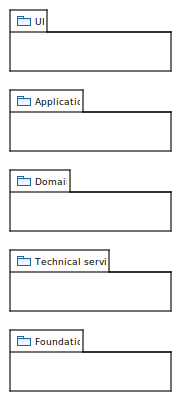
\includegraphics[width=0.3\textwidth]{img/layers.pdf}
    \caption{Paket-Diagramm der
        Player-Applikation}\label{fig:package-diagram:layers}
\end{figure}

\begin{figure}[H]
    \centering
    \includegraphics[width=0.9\textwidth]{img/player_package_diagram.png}
    \caption{Paket-Diagramm der Player-Applikation}\label{fig:package-diagram:player}
\end{figure}

\begin{figure}[H]
    \centering
    \includegraphics[width=1.0\textwidth]{img/editor_package_diagram.png}
    \caption{Paket-Diagramm der Editor-Applikation}\label{fig:package-diagram:editor}
\end{figure}

